% \date{May 14, 2024}
% \author{Deralive}
% \title{华东师范大学软件学院实验报告模板}
% 注意事项:编译两次,以确保目录、页码完整显示

\def\allfiles{}

%————————————多文件编译————————————%
% \ifx\allfiles\undefined
% 	    \begin{document}
% \else
% \fi

% Content

% \ifx\allfiles\undefined
% 	    \end{document}
% 	\else
% 	\fi
%—————————————————————————————————%

\documentclass[14pt,a4paper,UTF8,twoside]{article}

\usepackage{amsmath}
\usepackage{graphicx}
\usepackage{geometry} 
\usepackage{ctex}
\usepackage{booktabs} % 表格库
\usepackage{titlesec} % 标题库
\usepackage{fancyhdr} % 页眉页脚库
\usepackage{lastpage} % 页码数库
\usepackage{listings} % 代码块包
\usepackage{xcolor}
\usepackage[hidelinks]{hyperref}
\usepackage{tikz}
\usepackage{tikz-qtree}
\usepackage{fontspec} % 允许设置字体
\usepackage{unicode-math} % 允许数学公式使用特定字体
\usepackage{mwe}
\usepackage{zhlipsum} % 中文乱数文本
\usepackage{amsmath}
\usepackage{xcolor}
\usepackage{float} % 浮动体环境
\usepackage{subcaption} % 子图包
\usepackage{biblatex}
\usepackage{longtable}
\addbibresource{references.bib} % 指定你的.bib文件名称

\definecolor{mygreen}{rgb}{0,0.6,0}
\definecolor{mygray}{rgb}{0.5,0.5,0.5}
\definecolor{mymauve}{rgb}{0.58,0,0.82}

\date{} % 留空,以让编译时去除日期

%———————————————注意事项—————————————————%

% 1、如果编译显示失败,但没有错误信息,就是 filename.pdf 正在被占用
% 2、在文件夹中的终端使用 Windows > xelatex filename.tex 也可编译

%—————————————华东师范大学———————————————%

% 论文制作时须加页眉,页眉从中文摘要开始至论文末
% 偶数页码内容为:华东师范大学硕士学位论文,奇数页码内容为学位论文题目

%————————定义 \section 的标题样式————————%

% 注意:\chapter 等命令,内部使用的是 \thispagestyle{plain} 的排版格式
% 若需要自己加上页眉,实际是在用 \thispagestyle{fancy} 的排版格式
% 加上下面这一段指令,就能够让 \section 也使用 fancy 的排版格式
% 本质就是让目录、第一页也能够显示页眉、页脚

\fancypagestyle{plain}{
  \pagestyle{fancy}
}

\title{实验报告:Pintos Priority} % 模板
\titleformat{\section}
    {\normalfont\bfseries\Large} % 字体大小、字体系列(\bfseries 为加粗)
    {\thesection}{1em}{}

% 设置章节的中文格式
\renewcommand\thesection{\chinese{section} \hspace{0pt}}
\renewcommand\thesubsection{\arabic{subsection} \hspace{0pt}}
% \renewcommand\thesubsubsection{\alph{subsubsection} \hspace{0pt}} % 字母编号
% \hspace{0pt} 是为了确保在章节编号和章节题目之间不要有空格,使得排版更为美观
    
%—————————————页面基础设置———————————————%

\geometry{left=10mm, right=10mm, top=20mm, bottom=20mm}

%————————————设置页眉、页脚——————————————%

\pagestyle{fancy} % 设置 plain style 的属性

% 设置页眉

\fancyhead[RE]{\leftmark} % Right Even 偶数页右侧显示章名 \leftmark 最高级别章名
\fancyhead[LO]{\rightmark} % Left Odd 奇数页左侧显示节名 \rightmark 第二级别节名
\fancyhead[C]{华东师范大学软件工程学院学生实践报告} % Center 居中显示
\fancyhead[LE,RO]{~\thepage~} % 在偶数页的左侧,奇数页的右侧显示页码
\renewcommand{\headrulewidth}{1.2pt} % 页眉与正文之间的水平线粗细

% 设置页脚:在每页的右下脚以斜体显示书名

\fancyfoot[RO,RE]{\it Lab Report By \LaTeX} % 使用意大利斜体显示
\renewcommand{\footrulewidth}{0.5pt} % 页脚水平线宽度

% 设置页码:在底部居中显示页码

\pagestyle{fancy}
\fancyfoot[C]{\kaishu 第 \thepage 页 \ 共 \pageref{LastPage} 页} % LastPage 需要二次编译以获取总页数

%——————————————代码块设置———————————————%

\lstset {
    backgroundcolor=\color{white},   % choose the background color; you must add \usepackage{color} or \usepackage{xcolor}
    basicstyle=\footnotesize,        % the size of the fonts that are used for the code
    breakatwhitespace=false,         % sets if automatic breaks should only happen at whitespace
    breaklines=true,                 % sets automatic line breaking
    captionpos=bl,                   % sets the caption-position to bottom
    commentstyle=\color{mygreen},    % comment style
    deletekeywords={...},            % if you want to delete keywords from the given language
    escapeinside={\%*}{*},           % if you want to add LaTeX within your code
    extendedchars=true,              % lets you use non-ASCII characters; for 8-bits encodings only, does not work with UTF-8
    frame=single,                    % adds a frame around the code
    keepspaces=true,                 % keeps spaces in text, useful for keeping indentation of code (possibly needs columns=flexible)
    keywordstyle=\color{blue},       % keyword style
    % language=Python,               % the language of the code
    morekeywords={*,...},            % if you want to add more keywords to the set
    numbers=left,                    % where to put the line-numbers; possible values are (none, left, right)
    numbersep=5pt,                   % how far the line-numbers are from the code
    numberstyle=\tiny\color{mygray}, % the style that is used for the line-numbers
    rulecolor=\color{black},         % if not set, the frame-color may be changed on line-breaks within not-black text (e.g. comments (green here))
    showspaces=false,                % show spaces everywhere adding particular underscores; it overrides 'showstringspaces'
    showstringspaces=false,          % underline spaces within strings only
    showtabs=false,                  % show tabs within strings adding particular underscores
    stepnumber=1,                    % the step between two line-numbers. If it's 1, each line will be numbered
    stringstyle=\color{orange},      % string literal style
    tabsize=2,                       % sets default tabsize to 2 spaces
    % title=Python Code              % show the filename of files included with \lstinputlisting; also try caption instead of title
}

% 注释掉的部分用于后续插入代码,参数可调整,格式如下:

% 1、直接插入
% \begin{lstlisting}[language = ? , title = { ? } ]
%       Your code here.
% \end{lstlisting}

% 2、文件插入
% \lstinputlisting[language = C , title = ?.c] {filename.c}

%———————————————字体设置————————————————%

% \setCJKmainfont{SimSun} % 设置正文罗马族的 CJK 字体
% \renewcommand{\normalsize}{\fontsize{12pt}{15pt}\selectfont} % 设置正文字号
\linespread{1.2}

%——————————————————————————————————————%

%———————————————超链接设置——————————————%

\hypersetup{
    pdfstartview=FitH, % 设置PDF文档打开时的初始视图为页面宽度适应窗口宽度(即页面水平适应)
    CJKbookmarks=true, % 用对CJK(中文、日文、韩文)字符的书签支持,确保这些字符在书签中正确显示
    bookmarksnumbered=true, % 书签带有章节编号。这对有章节编号的文档很有用
    bookmarksopen=true, % 文档打开时,书签树是展开的,方便查看所有书签
    colorlinks, % 启用彩色链接。这样,链接在PDF中会显示为彩色,而不是默认的方框
    pdfborder=001, % 设置PDF文档中链接的边框样式。001 表示链接周围没有边框,仅在单击时显示一个矩形
    linkcolor=blue, % 设置文档内部链接(如目录中的章节链接)的颜色为蓝色
    anchorcolor=blue, % 设置锚点链接(即目标在同一文档内的链接)的颜色为蓝色
    citecolor=blue, % 设置引用(如文献引用)的颜色为蓝色
}

%——————————————导言区结束,进入正文部分———————————————%

%——————————————————————————————————————%

\begin{document}

\maketitle

\begin{center} % \extracolsep{\fill} 拉伸到页面最大宽度前,保证居中显示

  \begin{tabular*}{\textwidth}{@{\extracolsep{\fill}} l  l  l }
    \hline
    课程名称:操作系统 &  年级:2023级本科  &  上机实践成绩:\ \ \ \ \ \ \ \ \ \ \ \ \ \\
    指导教师:张民 & 姓名:张梓卫 \\
    上机实践名称:Pintos 忙等待问题 & 学号:10235101526 & 上机实践日期:2024/11/18 \ \ \ \ \ \ \ \ \ \ \ \ \ \\
    上机实践编号:(4) & 组号: & 上机实践时间:2 学时 \ \ \ \ \ \ \ \ \ \ \ \ \ \\
    \hline
  \end{tabular*}

\end{center}

\tableofcontents % 目录也需要二次编译

\section{实验目的}

本实验的目标是优化 Pintos 操作系统中的忙等待问题,
通过引入更加高效的调度和同步机制,以减少 CPU 的空转浪费并提高系统资源利用率。
传统的忙等待在资源不足或线程竞争时会导致 CPU 不断循环查询,既浪费了宝贵的处理资源,又可能阻塞其他线程的运行。

本次实验作出修改的代码如下所示:

同时上传到了 Github 之上,仓库地址为:\href{https://github.com/Shichien/ECNU-23-SEI-Homework/tree/main/%E6%93%8D%E4%BD%9C%E7%B3%BB%E7%BB%9F/%E5%AE%9E%E8%B7%B5%E8%AF%BE%E4%BD%9C%E4%B8%9A/Lec%202/lst2}{\underline{https://github.com/Shichien/ECNU-23-SEI-Homework}}

请在上传的 PDF 文件中直接点击粉色链接即可。

\section{内容与设计思想}



\section{使用环境}

使用 Docker v27.1.1 进行Pintos的安装实验,基于 Windows 11 操作系统使用 WSL2。

实验报告使用 \LaTeX 进行撰写,使用 VSCode + Vim 编辑器进行文本编辑。

\section{实验过程与分析}

\subsection{进入实验背景}

首先按照 PPT 的内容添加了 Printf 函数,显示
\begin{figure} [H]
    \centering
    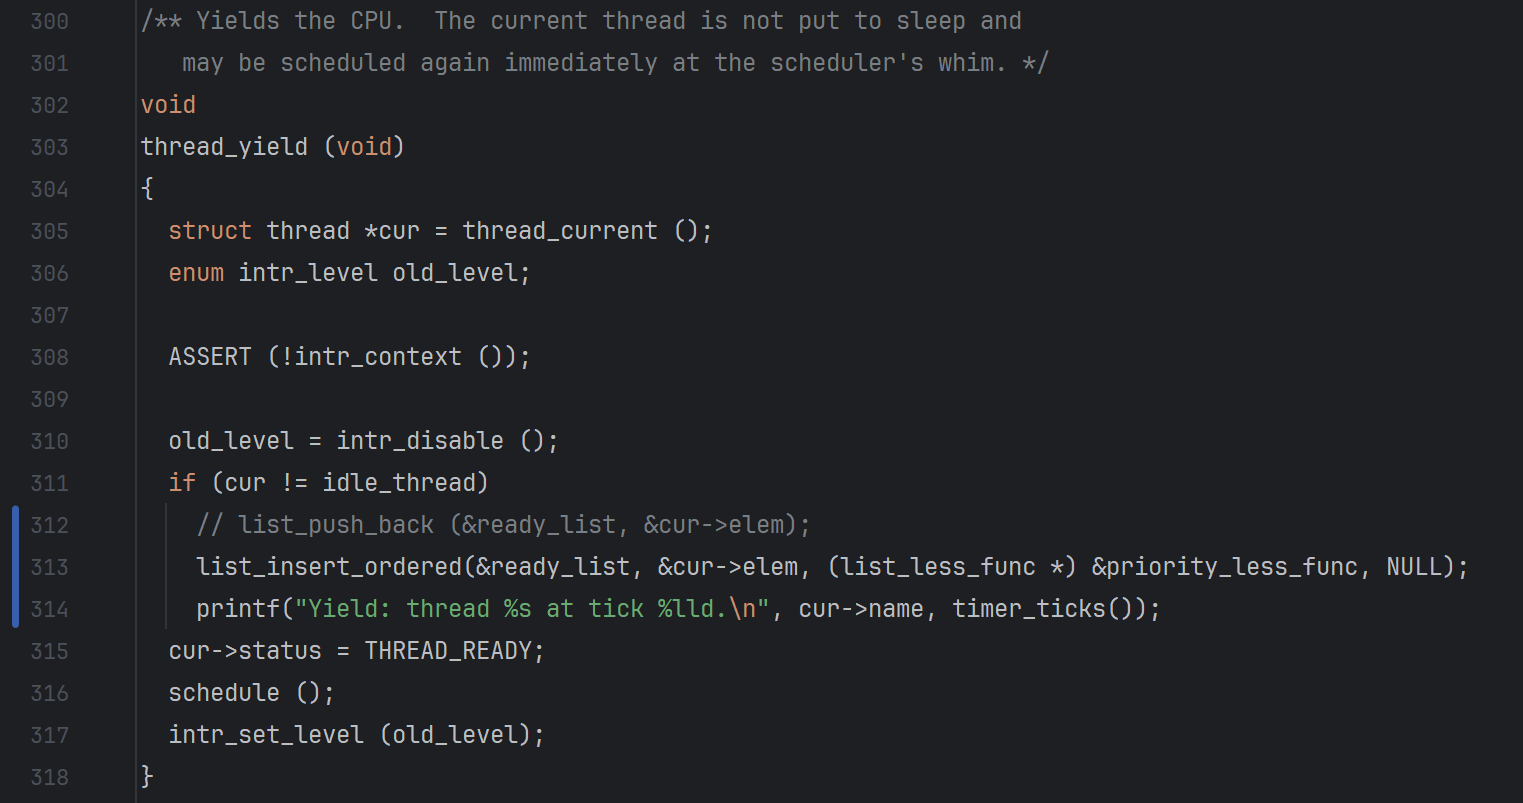
\includegraphics[width=0.8\textwidth]{img4/printf.png}
    \caption{添加 Printf 函数}
    \label{fig:pintos}
\end{figure}

最初忘记使用 Make 编译,所以修改代码后输出仍未发生改变,使用 Make 命令后,可以看到有了课件上相似的输出:

注意,这里的 Yield 刚开始打错了,后续在实验中进行了修改。
\begin{figure} [H]
    \centering
    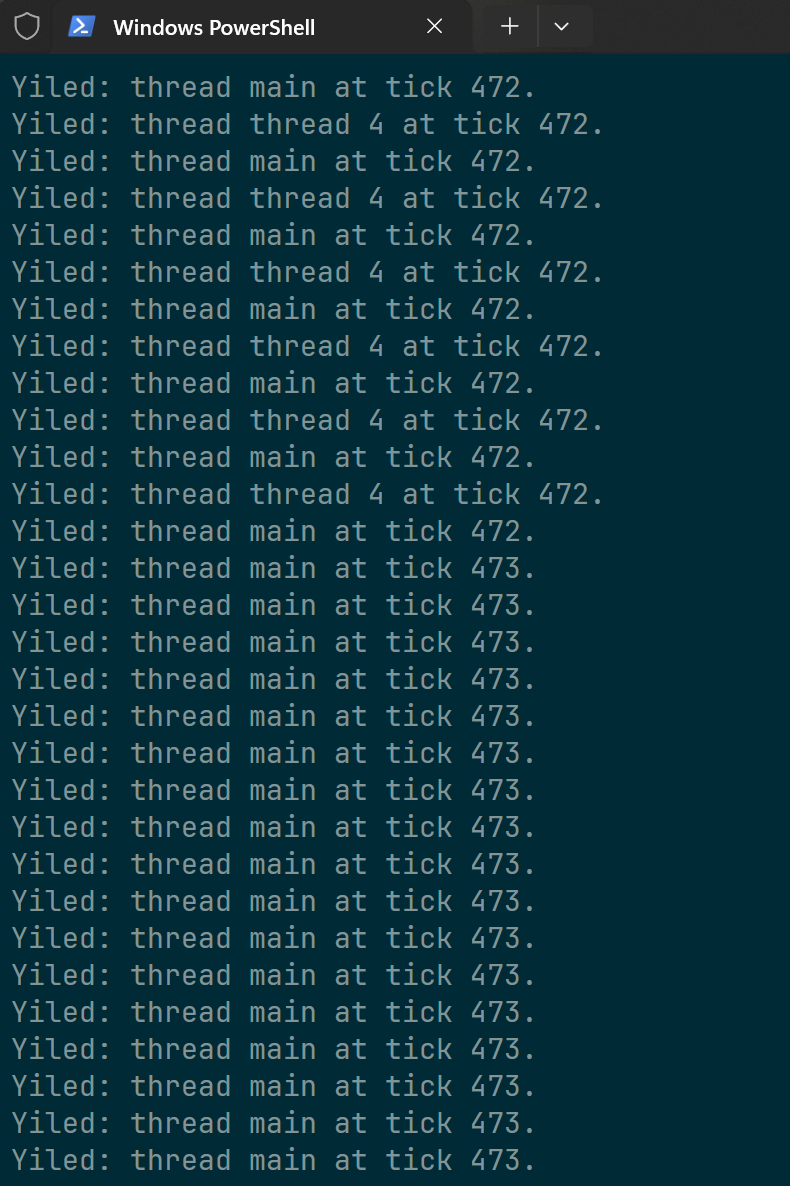
\includegraphics[width=0.3\textwidth]{img4/make.png}
    \caption{编译后输出}
    \label{fig:pintos}
\end{figure}

忙等待是一种线程或进程等待资源或条件时的方式。在忙等待期间,线程不断地通过循环检查条件是否满足,而不主动让出 CPU。这种行为导致线程虽然在逻辑上是“等待”,但实际上仍然占用 CPU 资源进行无效计算。

我们对输出的某些片段进行分析:

\begin{lstlisting}
Yield: thread main at tick 167.
Yield: thread thread 0 at tick 167.
Yield: thread thread 1 at tick 167.
Yield: thread thread 2 at tick 167.
Yield: thread thread 3 at tick 167.
Yield: thread thread 4 at tick 167.
...
Yield: thread main at tick 169.
Yield: thread thread 0 at tick 169.
Yield: thread thread 1 at tick 169.
Yield: thread thread 2 at tick 169.
Yield: thread thread 3 at tick 169.
Yield: thread thread 4 at tick 169.
\end{lstlisting}

主线程和多个子线程(thread 0 到 thread 4)在每个时钟周期(tick)内,都会多次输出 Yield。
线程没有实际执行任务,而是在轮流进行 yield 操作。这说明线程是在无条件地反复轮询,而没有进行有效的睡眠或释放 CPU 的操作。

在最后的片段中,如下:主线程在多个连续的 tick 内,不断重复同样的 Yield 输出。
同样,这表明主线程也在不停地轮询,等待某个条件满足。

\begin{lstlisting}
Yield: thread main at tick 564.
Yield: thread main at tick 564.
Yield: thread main at tick 564.
Yield: thread main at tick 564.
...
Yield: thread main at tick 570.
\end{lstlisting}

线程使用了 yield 语句,而不是睡眠或等待机制。
yield 的作用是将 CPU 时间片让给其他线程,但如果没有其他线程需要运行,则线程会立即重新获得 CPU 时间片并继续执行。这导致线程不断进入循环状态,占用 CPU。

\subsection{实现休眠}

\begin{figure}[H]
\centering
    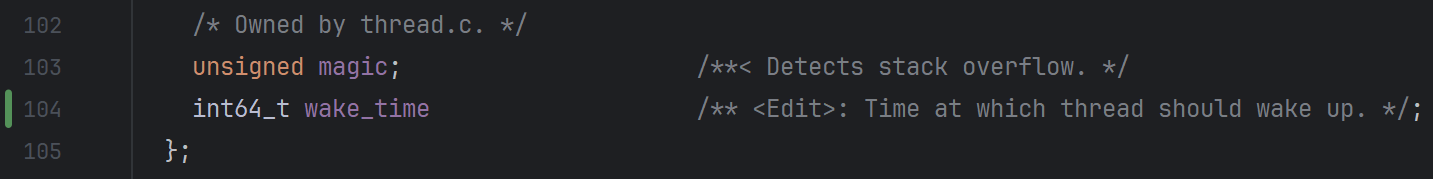
\includegraphics[width=0.5\textwidth]{img4/thread.png}
    \caption{修改 thread.h}
    \label{fig:pintos}
\end{figure}

\begin{figure}[H]
  \centering
  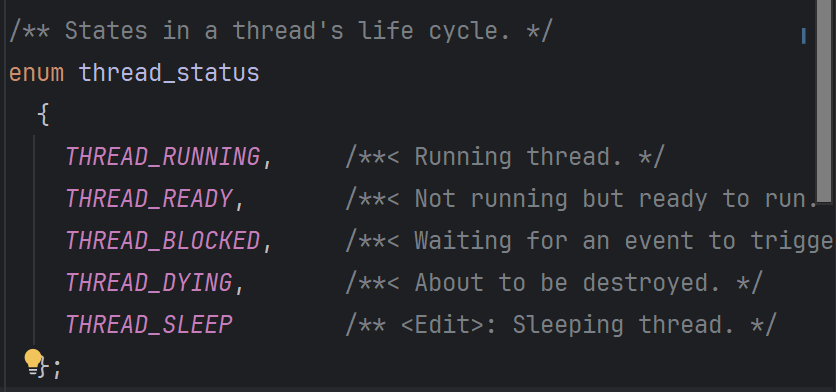
\includegraphics[width=0.4\textwidth]{img4/sleep_thread.png}
  \caption{修改 thread.h}
  \label{fig:pintos}
\end{figure}

在 thread.h 中,我们增加了 thread\_sleep 函数,定义休眠接口,供其他模块调用,用来让线程自身状态由运行状态转为休眠状态。

\begin{lstlisting}
  void thread_sleep(int64_t ticks);
\end{lstlisting}

在 thread.c 中,实现 thread\_sleep 函数。

\begin{lstlisting} [language = C]
void thread_sleep(int64_t ticks) {
	if(ticks<=0) return;
  	struct thread *cur = thread_current();

	enum intr_level old_level = intr_disable();
	if(cur!=idle_thread) {
  	cur->status = THREAD_SLEEP;
		cur->wake_time = timer_ticks() + ticks;
		schedule();
  }
	intr_set_level(old_level);
}
\end{lstlisting}

\begin{itemize}
  \item 检查休眠时间: 如果休眠时间 ticks 小于或等于 0,直接返回,不进行休眠。
  \item 获取当前线程: 调用 thread\_current() 获取当前线程的控制块 struct thread。
  \item 禁用中断: 禁用中断以保证线程状态和数据的修改是原子的,避免竞争条件。
  \item 线程状态更新:如果当前线程不是空闲线程(idle\_thread),将其状态设置为 THREAD\_SLEEP。
  \item 设置唤醒时间 wake\_time 为当前时钟计数加上休眠的 ticks。
  \item 调度:调用 schedule() 将线程切换出去,当前线程进入睡眠状态。
\end{itemize}

在 timer.c 中的 timer\_interrupt 函数中添加检查唤醒线程的逻辑。

定时器中断每次触发时,只检查需要唤醒的线程并唤醒它们,不进行不必要的轮询。
唤醒的线程重新参与调度后执行自己的任务。

\begin{figure}[H]
  \centering
  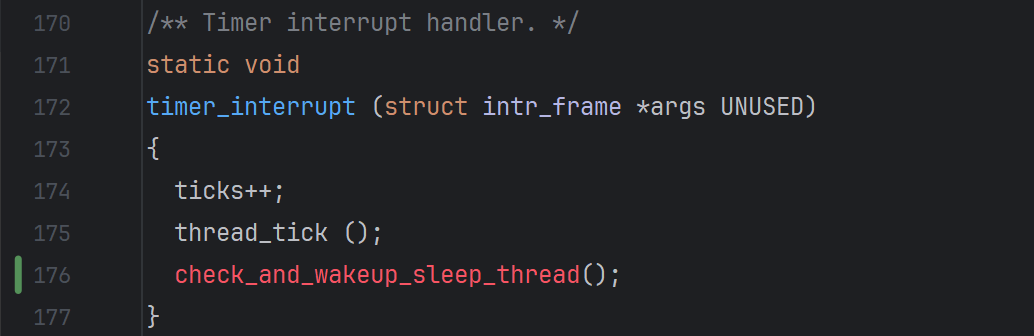
\includegraphics[width=0.4\textwidth]{img4/timer_interrupt.png}
  \caption{修改 timer.c}
  \label{fig:pintos}
\end{figure}

在 thread.c 中实现,同时与上同理,在 thread.h 中添加定义:

在调用 thread\_sleep 后,线程被阻塞并加入 sleep\_list,不再占用 CPU。
阻塞线程不会消耗任何 CPU 时间,而是等待时钟中断唤醒。

唤醒逻辑如下:

\begin{itemize}
  \item 获取当前时钟计数: 调用 timer\_ticks() 获取当前的时钟计数 cur\_ticks。
  \item 遍历所有线程: 遍历 all\_list 中的所有线程,找到状态为 THREAD\_SLEEP 且唤醒时间已到的线程。
  \item 更新线程状态:将满足条件的线程状态从 THREAD\_SLEEP 更新为 THREAD\_READY。
  \item 使用 list\_insert\_ordered 将线程加入 ready\_list,确保就绪队列按照优先级排序。
\end{itemize}

\begin{lstlisting} [language = C]
void check_and_wakeup_sleep_thread(void) {
	struct list_elem *e = list_begin(&all_list);
	int64_t cur_ticks = timer_ticks();

	while (e != list_end(&all_list)) {
		struct thread *t = list_entry(e, struct thread, allelem);
		enum intr_level old_level = intr_disable();
    if (t->status == THREAD_SLEEP && cur_ticks >= t->wake_time) {
        t->status = THREAD_READY;
        list_insert_ordered(&ready_list, &t->elem, (list_less_func *) &priority_less_func, NULL);
			  printf("Wake up thread %s at tick %lld.\n", t->name, cur_ticks);
		  }
    e = list_next(e);
		intr_set_level(old_level);
	}
}
\end{lstlisting}

在定时器中断(timer\_interrupt)中实现了对 sleep\_list 的轮询检查,将满足唤醒条件的线程从睡眠队列中移出并唤醒。

\subsection{解决忙等待}

再次输入命令\texttt{pintos -v -- -q run alarm-multiple},此时的输出如下所示:

这里只截取了一部分可以看出忙等待已经获得解决的输出:

\begin{figure}[H]
  \centering
  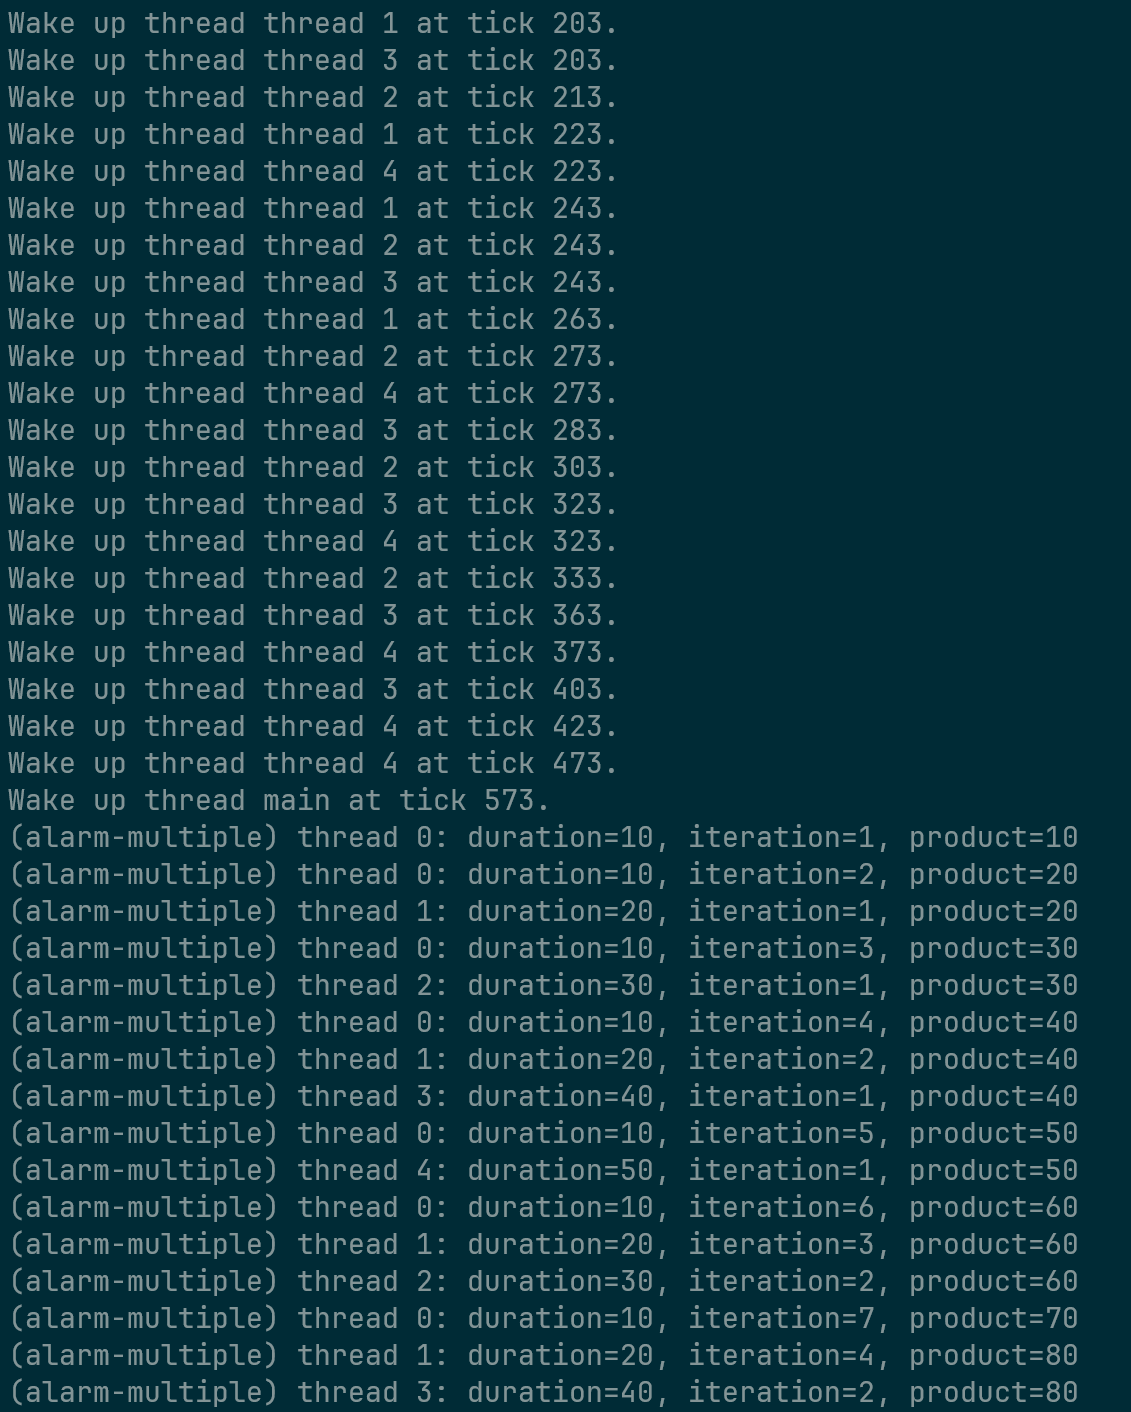
\includegraphics[width=0.45\textwidth]{img4/output.png}
  \caption{修改后的输出}
  \label{fig:pintos}
\end{figure}

\begin{lstlisting}
  Wake up thread thread 0 at tick 133.
  Wake up thread thread 1 at tick 143.
  Wake up thread thread 2 at tick 153.
\end{lstlisting}

日志显示线程只在预期的时间点(wakeup\_tick)被唤醒,每个线程只在需要执行任务时被唤醒,没有频繁轮询。

\begin{lstlisting}
(alarm-multiple) thread 0: duration=10, iteration=1, product=10
...
(alarm-multiple) thread 4: duration=50, iteration=7, product=350
\end{lstlisting}

在 alarm-multiple 日志中,每个线程只在被唤醒后完成一次任务,并再次进入睡眠。
日志显示的 product 值是单调递增的,表明线程按预期顺序执行,没有抢占或忙等待。

\subsection{实现苏醒后抢占}

其实,这部分只要在 check\_and\_wakeup\_sleep\_thread 函数中,
稍作修改即可,实现逻辑如下的注释所示:

\begin{lstlisting} [language = C, title= 苏醒后抢占]

bool check_and_wakeup_sleep_thread(void) {
    struct list_elem *e = list_begin(&all_list);
    int64_t cur_ticks = timer_ticks();
    bool need_preempt = false;

    while (e != list_end(&all_list)) {
        struct thread *t = list_entry(e, struct thread, allelem);
        if (t->status == THREAD_SLEEP && cur_ticks >= t->wake_time) {
            t->status = THREAD_READY;
            list_insert_ordered(&ready_list, &t->elem, priority_less_func, NULL);
            printf("Wake up thread %s at tick %lld.\n", t->name, cur_ticks);
            if (t->priority > thread_current()->priority) {
              // 判断是否需要抢占:
              // 如果被唤醒线程后,函数将其优先级与当前运行线程 (thread_current()) 的优先级进行比较。
              // 如果被唤醒线程的优先级更高,设置 need_preempt 为 true,表示需要进行上下文切换,以便高优先级线程立即运行。
                need_preempt = true;
            }
        }
        e = list_next(e);
    }
    return need_preempt;
}

\end{lstlisting}

在这个函数里,使用了 \texttt{list\_insert\_ordered(\&ready\_list, \&t->elem, priority\_less\_func, NULL);}

确保线程按照优先级从高到低排列,因此 ready\_list 的第一个线程始终是优先级最高的线程。

另外,我们需要调用这个函数,在 thread\_tcik 中检查,如果返回 true,则调用 intr\_yield\_on\_return() 来进行上下文切换
\begin{lstlisting} [language = C, title= 苏醒后抢占]
  void
thread_tick (void)
{
  struct thread *t = thread_current ();

  /* Update statistics. */
  if (t == idle_thread)
    idle_ticks++;
#ifdef USERPROG
  else if (t->pagedir != NULL)
    user_ticks++;
#endif
  else
    kernel_ticks++;

	/* Check if the current thread needs to be woken up. */
	bool need_preempt = check_and_wakeup_sleep_thread();

  /* Enforce preemption. */
  if (++thread_ticks >= TIME_SLICE || need_preempt) {
	printf("Tick: thread %s at tick %lld.\n", t->name, timer_ticks());
  // 为了能够看出是否实现了苏醒后抢占,我们可以添加一些提示信息
    intr_yield_on_return ();
  }
}
\end{lstlisting}

这一次输出片段如下:

\begin{lstlisting} [language = C]
Tick: thread idle at tick 213.
Yield: thread idle at tick 213.
Wake up thread thread 1 at tick 223 (priority=31).
Thread thread 1 will preempt current thread idle.
Wake up thread thread 4 at tick 223 (priority=31).
Thread thread 4 will preempt current thread idle.
Tick: thread idle at tick 223.
Yield: thread idle at tick 223.
Wake up thread thread 1 at tick 243 (priority=31).
Thread thread 1 will preempt current thread idle.
Wake up thread thread 2 at tick 243 (priority=31).
Thread thread 2 will preempt current thread idle.
Wake up thread thread 3 at tick 243 (priority=31).
Thread thread 3 will preempt current thread idle.
\end{lstlisting}

可以看到,线程 1 到 4 都被唤醒,并且在被唤醒后,线程 1 开始运行,而线程 4 则被抢占,以便线程 1 运行。


\subsection{实验结果}

\begin{figure}[H]
  \centering
  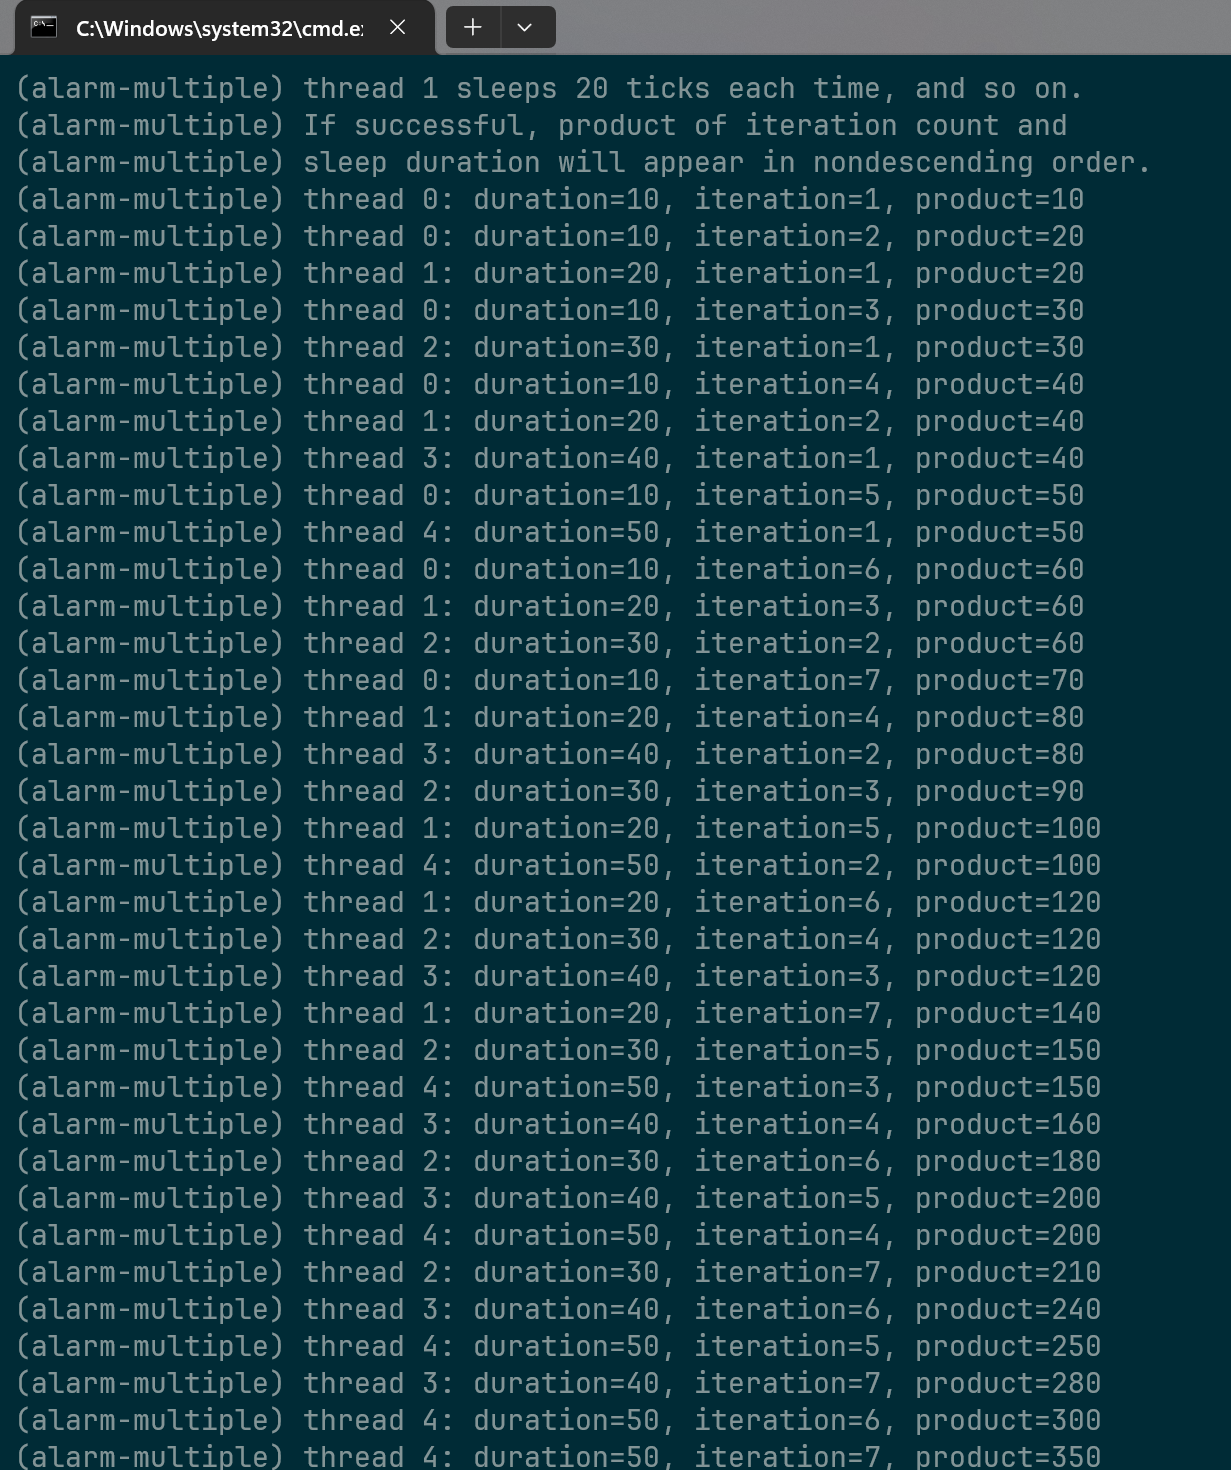
\includegraphics[width=0.5\textwidth]{img4/final.png}
  \caption{实验结果}
  \label{fig:pintos}
\end{figure}

最后的 "product" 消息显示线程完成其睡眠循环的顺序。
乘积值的非降序顺序表明线程根据其睡眠持续时间和优先级按正确顺序被唤醒和执行。


\section{总结}

\subsection{实验成果}

\begin{enumerate}
    \item \textbf{实现线程休眠}  
    \begin{itemize}
        \item 在 \texttt{thread.c} 中实现了 \texttt{thread\_sleep()} 函数,使线程在不需要执行任务时进入休眠状态,并在唤醒时间到达时由定时器中断恢复运行。
        \item 休眠机制避免了线程频繁调用 \texttt{thread\_yield()} 导致的资源浪费,使得线程在等待资源时不会占用 CPU,显著提高了资源利用效率。
    \end{itemize}

    \item \textbf{实现线程唤醒}  
    \begin{itemize}
        \item 通过修改 \texttt{check\_and\_wakeup\_sleep\_thread()} 函数,定时器中断在适当的时刻检查所有线程,并将符合条件的线程从睡眠队列移动到就绪队列,同时更新其状态为 \texttt{THREAD\_READY}。
        \item 这一机制确保了线程仅在需要时被唤醒,进一步减少了不必要的 CPU 开销。
    \end{itemize}

    \item \textbf{实现苏醒后抢占}  
    \begin{itemize}
        \item 在线程唤醒的逻辑中,我们比较唤醒线程与当前运行线程的优先级。如果唤醒线程的优先级更高,则触发抢占,使高优先级线程得以优先运行。
        \item 这一机制提升了操作系统的实时性和响应性,使得优先级调度策略得以有效执行。
    \end{itemize}
\end{enumerate}

\subsection{附录}

\textbf{参考资料}:

\begin{itemize}
    \item \href{https://pkuflyingpig.gitbook.io/pintos/project-description/lab1-threads/faq}{\underline{https://pkuflyingpig.gitbook.io/pintos/project-description/lab1-threads/faq}}
\end{itemize}

\end{document}